\documentclass[12pt]{article}
\usepackage{graphicx} % Required for inserting images
\usepackage{caption}
\usepackage{subcaption}
\usepackage{float}

\title{What were the initial conditions of the early universe that promoted the growth of structure we see today?}
\author{Dhanush Ekollu}
\date{April 2023}

\begin{document}

\maketitle

\section{Inflation}
Our current standard Big Bang Theory defines gradual growth throughout the universe’s lifetime. While this theory explains many things such as the CMB’s blackbody spectrum, it has 3 significant issues: The Horizon Problem, The Flatness Problem, and The Magnetic Monopole Problem. 

Inflation Theory proposes that the universe had a short period of extreme, rapid growth following its birth–lasting from $10^{-36}$ seconds after the Big Bang singularity to between $10^{-33}$ seconds and $10^{-32}$ seconds after the singularity. After this period of exponential expansion, the universe expanded at a slower pace.

The Horizon Problem presents that the universe possesses a background temperature that is unexpected. There was not enough time for the universe to equilibrate because the expansion would move parts of the universe away faster than light. Consequently, those parts would never interact with each other to equalize to the same background temperature. Despite that, every new part of the universe that we see (as their photons reach us for the first time) has the same properties as our part. Inflation, if it occurred, would explain this discrepancy. If the universe was very small, particles could equilibrate at that time and have a background temperature, and then the universe would expand at a more rapid rate. 

The Flatness Problem is that it is extraordinarily unlikely for the universe to be flat as it is now–the universe would have to be at the perfect critical density and require the perfect initial conditions. Inflation solves this problem because it stretches the curvature of the universe to make it very flat.

Finally, the Magnetic Monopole Problem questions why no magnetic monopoles can be found, despite a considerable number of stable magnetic monopoles that should have formed in the early universe. Inflation does not rule out their existence, but it solves this problem by stating that the magnetic monopoles produced in the early universe would be pushed very far apart, and their perceived density would reduce significantly once the universe's temperature became too cool to produce new ones.

Inflation also explains why we see large-scale structures today. Since there was a period of immense exponential expansion when the universe was born, anything not bound together expanded along with it. Small quantum fluctuations during this period of inflationary expansion were greatly amplified and gravity further exacerbated these overdensities, causing large-scale structure today like galaxy superclusters. Thus, Inflation theory solves the 3 aforementioned cosmological problems, explains why there are large-scale structures today, and also clarifies why few inhomogeneities remain in the universe’s density and curvature. However, Inflation is just a theory as of now–one that can be proved with very precise measurements of the Cosmic Microwave Background (CMB).

\section{The Cosmic Microwave Background}
The CMB is microwave relic radiation left over from the big bang and is a nearly perfect blackbody. It is the result of an event in the universe called recombination. The CMB serves as a powerful tool to understand the initial conditions of the universe and all significant events that have occurred since its formation.

Before recombination, photons, electrons, and baryons formed a photon-baryon fluid. Free electrons glued these photons to baryons. Baryons would follow electrons and CMB photons would not travel far before Thomson Scattering off an electron because of the density and heat of the universe back then. This photon-baryon plasma had pressure, supplied by the radiation itself. Just like a gas under pressure, it fights against it, bounces back bigger than it originally was (Compression), and then shrinks back to its original size (Rarefaction). These caused sound waves/acoustic oscillations in the CMB.

Going backward in time, when the universe was 1/1000th times its current size, it was a thousand times hotter. There was enough energy back then for hydrogen atoms to be broken into protons and neutrons. Going forward in time, that means that neutral hydrogen atoms were first formed then (after the universe cooled down enough). This process is called recombination. It occurred only 300,000 years after the universe’s birth and the CMB was formed at this point. Since the universe is almost 10 billion years old, the CMB is a record of the universe since virtually its very beginning.

Due to this, the CMB contains vital information about the events that took place in the early universe, its history, and its properties. As we look further into the CMB, we see that even though it is very homogenous, anisotropies do exist. These temperature anisotropies directly correlate with large-scale structure in the universe–there is a higher density of galaxies in hot patches and a far lower density in cold patches. The first peak in the temperature spectrum contains information about the curvature of the universe, the second peak shows us the amount of matter in the universe and the higher peaks like the third peak define the dark matter density. 

Different conditions like the universe being matter dominated instead of energy-dominated change the peaks’ properties (by increasing their amplitude, for example). This can show us when the universe went through its different stages. We can also find the matter density, because the higher it is, the more CMB photons/baryons bounce around before recombination, shifting damping tails to higher multipoles. Many of the same factors found in the temperature spectrum can also be found in the damping tails, so they provide consistency checks to double-check our assumptions.

However, many cosmological properties make the same changes as others on the CMB’s power spectrum. Because of this, it can be uncertain which parameter caused what we see. Fortunately, polarizations are another invaluable tool in the CMB that can be used to break the parameter degeneracy. They are the most direct way to look at the conditions after recombination and later reionization. Commonly found E-mode polarizations (parallel/perpendicular to up/down) provide information about lots of historic cosmic events since most form them. B-modes (crossed at 45-degree angles) are a lot rarer and significantly harder to detect. These can prove Inflation theory because the gravitational waves that inflation would have caused would leave their mark on the CMB as B-mode polarizations. 

The CMB is both a map of the universe and a timeline of its historic events. It also contains an imperative way to prove Inflation theory, solving many of the current cosmological problems that daunt cosmologists today.

\section{Methods}
% REWRITE!!!
First, I took data from NASA CAMB and the Atacama Cosmology Telescope (ACT) and filtered it using standard filtering techniques such as Fourier Transforms, Convolutions, etc. I then used the filtered data to plot maps of the CMB’s power spectrum, a temperature anisotropy map, and other visualizations of the CMB. I experimented with various noise and atmospheric effects such as frequency dependence to demonstrate the effects these have on the calculated power spectrum. After testing many common tools on CMB measurements, I generated a simulation of the universe’s CMB if it had different parameters such as curvature using NASA LAMBDA CAMB.

I used this to visualize polarization in the CMB and simulate B-mode polarizations, along with the B-mode power spectrum. I also analyzed the different scientific and instrumental phenomena that cause discrepancies and inaccuracies while taking measurements of the CMB–including but not limited to SZ maps, instrument beams, white noise, diffraction, and atmospheric noise. I plan to simulate different values of r (the tensor-to-scalar ratio) for B-mode polarizations as a way to simulate the inflationary expansion rate. If r is too low, instruments would be unable to pick up the signal from B-mode polarizations, prohibiting us from studying them and the vast array of knowledge they contain. Finally, I also hope to demonstrate the difference between a B-mode power spectrum for inflation versus due to gravitational lensing. Gravitational lensing appears as B-mode polarizations but are actually recent polarizations and do not contain the information we are looking for, so they must be filtered.

\section{Results and Analysis}
For these results, I used Jeff McMahon’s notebooks prepared for the CMB Analysis Summer School held at the University of Michigan. I was able to replicate most of the notebook’s results successfully.

\subsection{NASA LAMBDA CAMB}
Firstly, I tested various analysis tools and math functions that are frequently used while working with the CMB on a simulated version of our universe from NASA LAMBDA CAMB. After successfully replicating the results of the notebook on the simulated universe, I went on to use these tools on public telescope data from the Atacama Cosmology Telescope. 

To begin, I generated a power spectrum and temperature anisotropy map for the simulated CAMB universe with the data CAMB itself provided, shown in Figure \ref{fig:fs} and Figure \ref{fig:camb_temp}. The area rendered for the map was a small patch of the sky made by generating a 2D power spectrum by revolving the above power spectrum, generating a Gaussian random map, multiplying the 2 maps, and using a Fourier transform to get a real space map.

\begin{figure}[H]
    \centering
    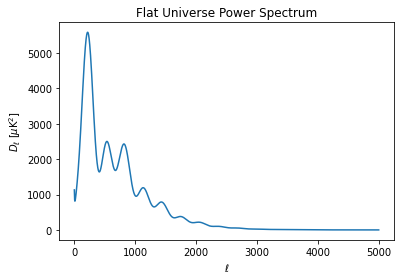
\includegraphics[width=0.6\textwidth]{images/fs.png}
    \caption{The angular power spectrum generated for the simulated CAMB universe, which matches the well-known and recognizable CMB power spectrum.}
    \label{fig:fs}
\end{figure}

\begin{figure}[H]
    \centering
    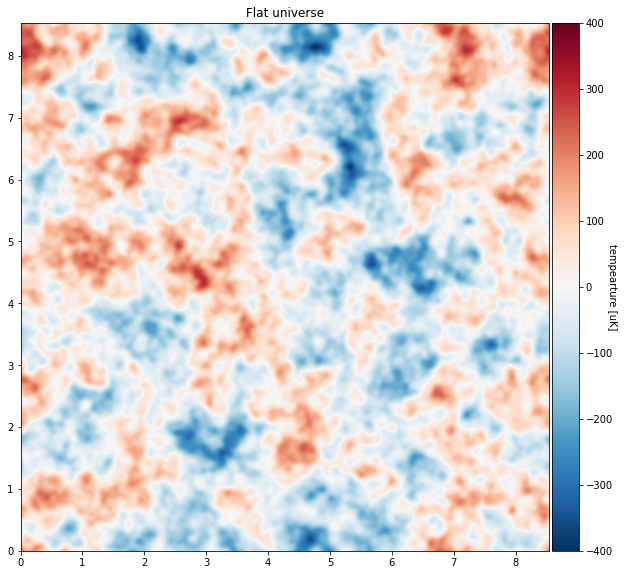
\includegraphics[width=0.6\textwidth]{images/fa.png}
    \caption{A temperature anisotropy map also generated from the simulated CAMB data, which matches the previous results of the notebook. The area rendered was a small patch of the sky made by revolving the above power spectrum, a Gaussian random map, multiplying the 2 maps, and using a Fourier transform.}
    \label{fig:camb_temp}
\end{figure}

To more realistically emulate a telescope’s reading of the CMB instead of the perfect data from NASA CAMB, I simulated the various forms of noise that usually arise while measuring data of the CMB. First, a few forms of common astrophysical noise were generated. A Point Source Map (Figure \ref{fig:point_source_map}) was simulated–with some of the astrophysical objects approximated as a combination of faint sources and a few very bright sources. The sources were chosen to look like a real map at 150 GHz. Point Sources are very useful for calibrating telescopes and are useful for other data analysis on the CMB, but they will be filtered out for our purposes. Then, an SZ map (Figure \ref{fig:sz_map}) was simulated by fixing each cluster to an identical angular size. SZ maps (the Sunyev-Zeldovich effect) is when the dilute gas which is at a temperature of millions of kelvin in clusters of galaxies imprint subtle distortion into the CMB map by interacting with a CMB photon and giving it a boost in energy. For better simulations, a range of cluster sizes should be used. I generated a full sky map that contains the detected CMB Anisotropies with the added noise from astrophysical noise.

To account for telescope diffraction, I convolved the map with a Gaussian beam pattern with an FWHP = 1.25 degrees. I then added several types of noise such as white noise (10 $\mu$K-arcmin) drawn from a Gaussian distribution, atmospheric noise which grows larger on large angular scales, and $1/f$ noise in the detectors. White noise contains an equal amount of energy across all frequencies, while $1/f$ noise has more power at lower frequencies and less at higher frequencies. Atmospheric noise is noise from sources like water vapor, turbulence due to high altitude, etc. Telescopes are usually turned off when water vapor is too high due to a storm because the vapor can interfere with the microwave radiation by absorbing and re-emitting it. See figure \ref{fig:instrument_noise} for instrument noise map.

Finally, I added these noise maps and the simulated convolved sky map to generate a complete simulated CMB map (Figure \ref{fig:complete_map}) including all key astrophysical and instrumental effects. I was able to fully replicate this result as demonstrated in the notebook.

\begin{figure}[h]
     \centering
     \begin{subfigure}[t]{0.3\textwidth}
         \centering
         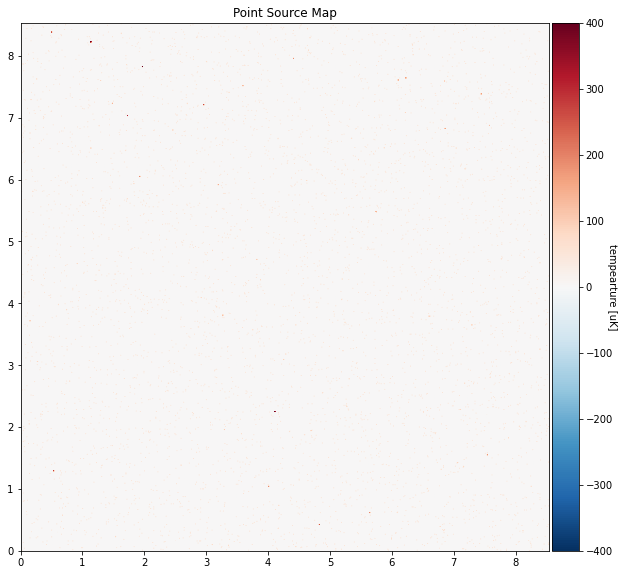
\includegraphics[width=\textwidth]{images/point source map.png}
         \caption{Point Source Map}
         \label{fig:point_source_map}
     \end{subfigure}
     \hfill
     \begin{subfigure}[t]{0.3\textwidth}
         \centering
         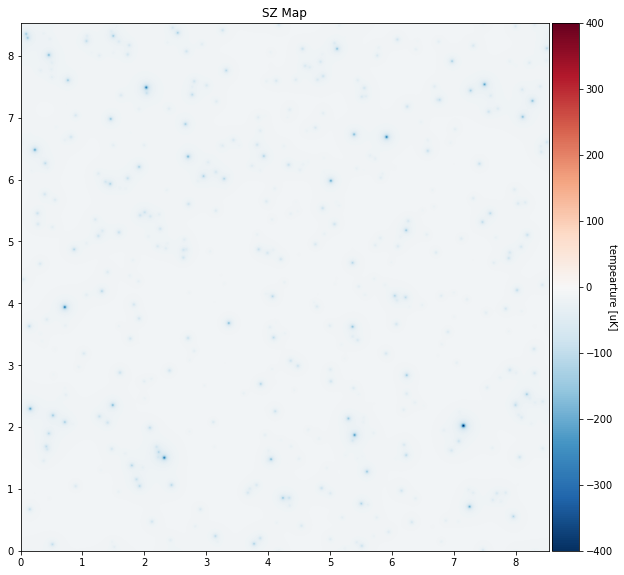
\includegraphics[width=\textwidth]{images/SZ map.png}
         \caption{SZ Map}
         \label{fig:sz_map}
     \end{subfigure}
     \hfill
     \begin{subfigure}[t]{0.3\textwidth}
         \centering
         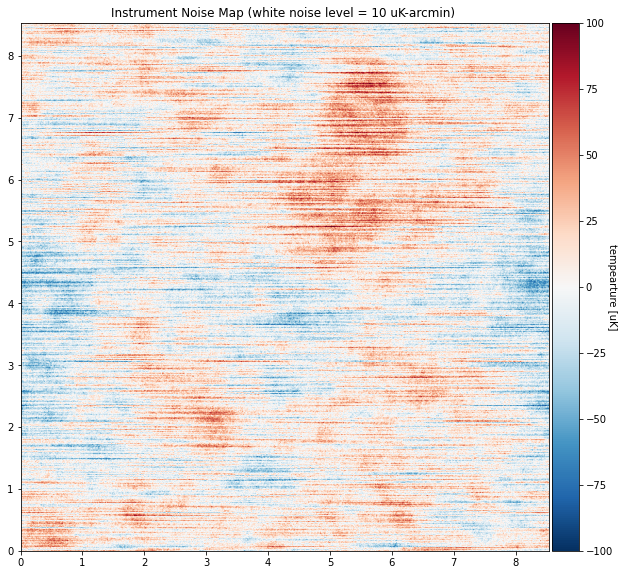
\includegraphics[width=\textwidth]{images/Instrument noise.png}
         \caption{Instrument Noise}
         \label{fig:instrument_noise}
     \end{subfigure}
        \caption{Various Noise Maps}
        \label{fig:my_label}
\end{figure}

\begin{figure}[H]
    \centering
    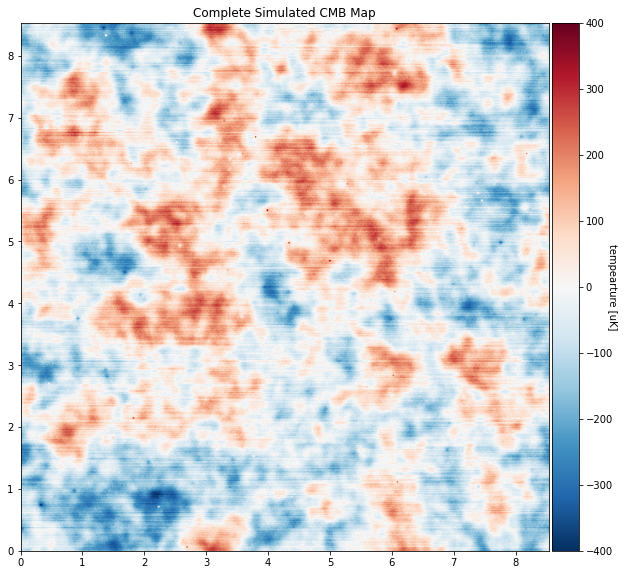
\includegraphics[width=\textwidth]{images/complete simulated CMB Map.png}
    \caption{The complete simulated CMB sky map, with all key astrophysical and instrumental effects added on top of the temperature anisotropy map.}
    \label{fig:complete_map}
\end{figure}

Next, I computed the power spectrum from the CMB Map, working in the same flat sky approximation (treating the celestial sphere as a flat plane for the purpose of mathematical calculations and analysis) as before when the simulated CMB Map was generated. A CMB map itself is not very useful in understanding deeper physics, but it is an excellent first tool in understanding how noise affects the true reading of the CMB and how to mitigate its effects with the appropriate filtering tools. Once the map is filtered, it can be used to generate a power spectrum which is much more useful and amplifies the power of the CMB signal with little noise. The peaks of the power spectrum contain vital information about the universe, so it is crucial to get as accurate of a reading as possible of the CMB signal. Before taking a 2D Fast Fourier Transform (FFT), I experimented with various windows to apodize the map and eliminate edge effects, avoiding spurious signals. A 2D FFT is usually the obvious thing to do when calculating a power spectrum and is a mathematical operation which is used to transform a two-dimensional spatial domain signal or image into its frequency domain representation. Apodizing a map is where a function is used to smooth off the edges of a map and filter out unwanted artifacts. A cosine window was implemented first, in Figure \ref{fig:cosine_window}.

\begin{figure}[H]
    \centering
    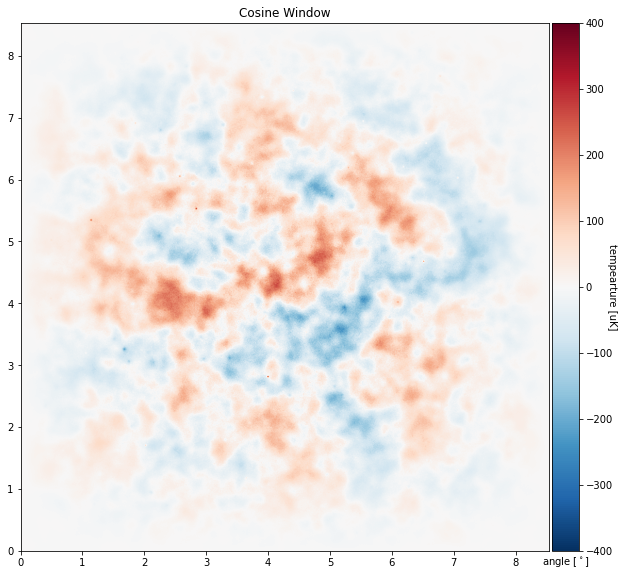
\includegraphics[width=0.6\textwidth]{images/cosine.png}
    \caption{The map after a cosine window was used to apodize it. While the cosine window rounds off the edges, it also suppresses the signal a significant amount.}
    \label{fig:cosine_window}
\end{figure}

I also tried out other windows such as a sine window (Figure \ref{fig:sine_window}) and a sine squared window (Figure \ref{fig:sine_squared_window}). These windows resulted in predictable and expected parts of the map that became suppressed due to the nature of the functions and their graphs.

\begin{figure}[H]
     \centering
     \begin{subfigure}[t]{0.49\textwidth}
         \centering
         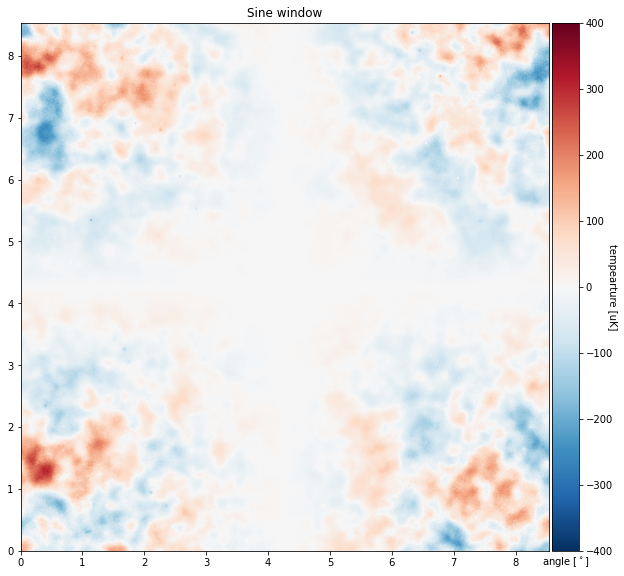
\includegraphics[width=\textwidth]{images/sine.png}
         \caption{A sine window. The effects of this window on the map are expected as graph $y=\sin\theta$ is shifted from the cosine graph.}
         \label{fig:sine_window}
     \end{subfigure}
     \hfill
     \begin{subfigure}[t]{0.49\textwidth}
         \centering
         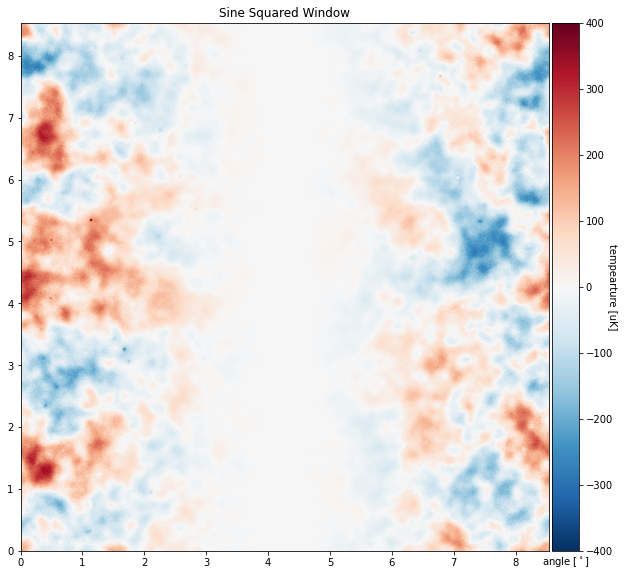
\includegraphics[width=\textwidth]{images/sine squared.png}
         \caption{A sine squared window. The effects of this window on the map are also fairly predictable since the suppressed part of the map is now thinner and no longer horizontal as well. The graph $y=\sin^2\theta$ is steeper and positive throughout.}
         \label{fig:sine_squared_window}
     \end{subfigure}
        \caption{Various windows}
        \label{fig:my_label}
\end{figure}

Next, I computed a naive power spectrum (Figure \ref{fig:naive}) and compared it to the input power spectrum used for the simulations. This power spectrum is computed by applying a 2D FFT, taking the absolute value squared of the map in Fourier space, and averaging the signal in annular bins of $k = \sqrt{k_x^2 + k_y^2}$.  These bins are converted to bins in $\ell$ with the scaling: $\ell = k* 2 \pi$ per the flat sky approximation.

\begin{figure}[H]
    \centering
    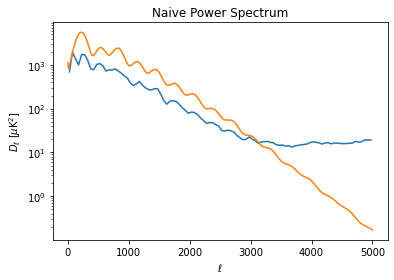
\includegraphics[width=0.6\textwidth]{images/Naive Power Spectrum.png}
    \caption{The naive power spectrum (blue) and the input CMB power spectrum (orange). The naive power spectrum varies due to the added instrumental and astrophysical noise such as SZ Maps and point source signals, along with suppression from the beam and apodization.}
    \label{fig:naive}
\end{figure}

The importance of a good window function is highlighted here. While window functions take away edge cases, they also lose important info about the power spectrum when the window function is too powerful. A balance between a window function and raw data is therefore crucial.

Next, I corrected the additive and multiplicative bias to get an unbiased estimate of the measured spectrum $\hat{D_\ell}$ to the true spectrum $D_\ell$.
$$\hat D_\ell = T*D_\ell + N. $$
The true power spectrum can be recovered using monte carlo techniques, using simulations to compute $T$ (transfer function of the instrument and filtering) and $N$ (additive noise term) and then using algebra to correct the naive measurement. This can be expressed in an equation as follows:
$$ D_\ell = \hat (D_\ell - N)/T. $$
The transfer function was calibrated by generating sky simulations with a known power spectrum, modeling the transfer function of the instrument and the post-processing, keeping the noise level to 0, and calculating the naive power spectrum for each simulation. Many simulations were run to reduce numerical noise and finally, the true spectrum was divided by the average signal-only spectrum to recover the estimate for the transfer function. 64 realizations were used in this example, and the accuracy increases as the number of realizations does. All of this was done following the notebook's example, and I replicated the same power spectrum results as the notebook, shown in Figure \ref{fig:naive_spectrums}

\begin{figure}[H]
    \centering
    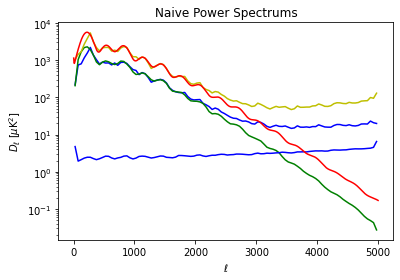
\includegraphics[width=0.6\textwidth]{images/naive spectrums.png}
    \caption{The estimate of the CMB power spectrum after correcting for multiplicative bias (yellow), the input power spectrum (red), the average of the signal only simulations (green), the transfer function (blue, lower), and the naive power spectrum (blue, upper).}
    \label{fig:naive_spectrums}
\end{figure}

The noise bias is then calibrated by running noise-only simulations through the naive power spectrum estimator and computing the average power spectrum. The error bars are computed by generating simulations including signal and noise, computing the naive power spectrum, taking the Root Mean Square of these results, and subtracting the noise bias and accounting for the transfer function. The final computed CMB Power Spectrum with error bars is shown in Figure \ref{fig:computed_cmb}

\begin{figure}[H]
    \centering
    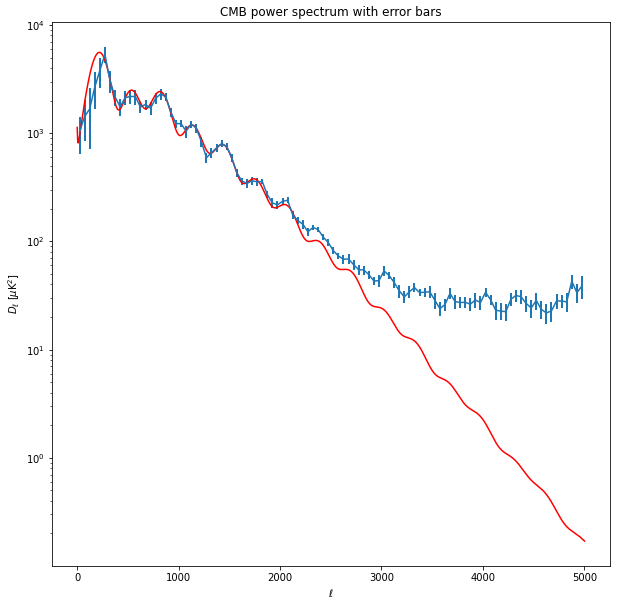
\includegraphics[width=0.8\textwidth]{images/cmb error bars.png}
    \caption{A computed CMB Power spectrum with error bars}
    \label{fig:computed_cmb}
\end{figure}

With all the tools and notebook code tested on simulated telescope data from NASA CAMB, I went on to use real public telescope data from the ACT collaboration.

\subsection{ACT Telescope Data}
To start off, I read the public data from the Atacama Cosmology Telescope provided in the GitHub repository of the notebook, shown in Figure \ref{fig:reading}.

\begin{figure}[H]
    \centering
    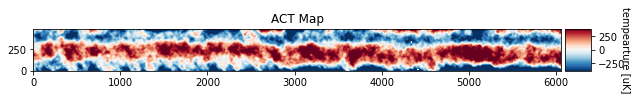
\includegraphics[width=0.8\textwidth]{images/ACT Map.png}
    \caption{ACT Map - 148 GHz}
    \label{fig:reading}
\end{figure}

Since the ACT Map is a long stripe, I cut out a patch of it and computed the power spectrum on that first. I took a cosine window on the patch and then plotted the apodized map. I then used the same filtering techniques on this map as with the simulated noise on the CAMB map. Finally, I took the power spectrum on the apodized map and compared it to the theoretical power spectrum.

\begin{figure}[H]
     \centering
     \begin{subfigure}[t]{0.49\textwidth}
        \centering
        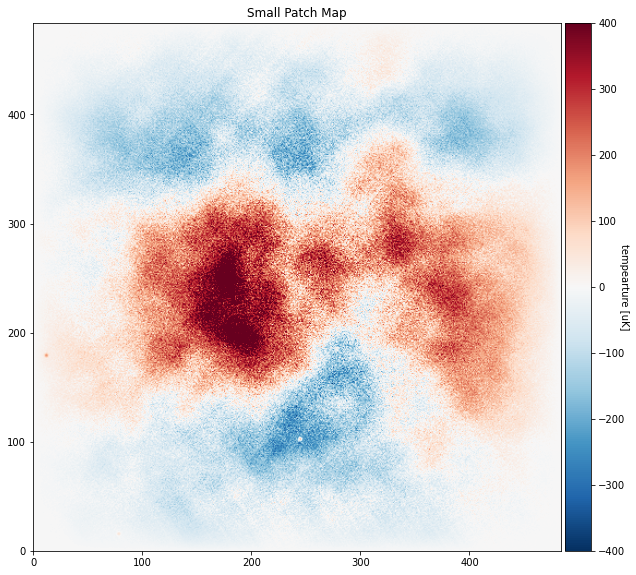
\includegraphics[width=0.7\textwidth]{images/ACT Map Patch.png}
        \caption{ACT sky map for a small patch of the reading. There is a lot of power from large scales from the atmosphere, so the power spectrum generated from the data can be expected to be biased to higher scales.}
        \label{fig:my_label}
     \end{subfigure}
     \hfill
     \begin{subfigure}[t]{0.49\textwidth}
        \centering
        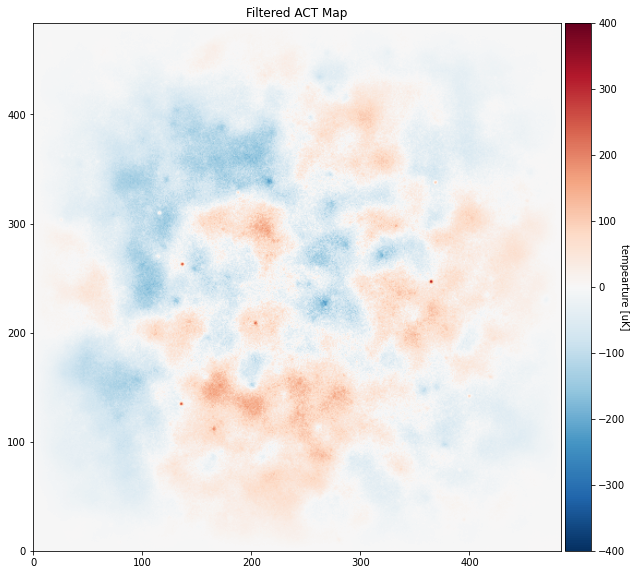
\includegraphics[width=0.7\textwidth]{images/Filtered ACT Map.png}
        \caption{ACT Map Patch filtered with same techniques as simulated CAMB map.}
        \label{fig:my_label}
     \end{subfigure}
        \caption{ACT Map Patches, Unfiltered and Filtered}
        \label{fig:my_label}
\end{figure}

\begin{figure}[H]
    \centering
    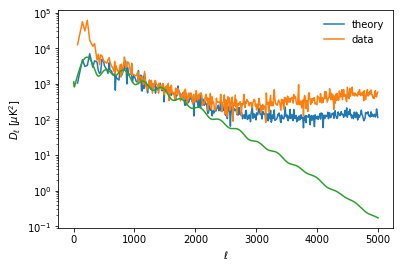
\includegraphics[width=0.8\textwidth]{images/ACT PS.png}
    \caption{Power Spectrum Generated from Data vs Theoretical Power Spectrum}
    \label{fig:my_label}
\end{figure}

I also tested the frequency dependence of maps and foregrounds by looking at ACT Maps generated from the same patch of the sky but in a different frequency band (at 220 GHz instead of the previous 148 GHz) and calculating a power spectrum from that data using the same method.

\begin{figure}[H]
    \centering
    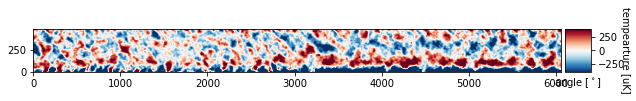
\includegraphics[width=0.8\textwidth]{images/diff fb act.png}
    \caption{ACT Map - 220 GHz}
    \label{fig:my_label}
\end{figure}

\begin{figure}[H]
    \centering
    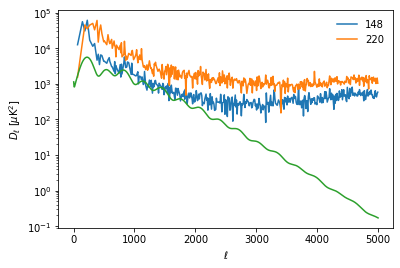
\includegraphics[width=0.8\textwidth]{images/PS 220.png}
    \caption{Power spectrum generated at 220 GHz vs the power spectrum generated and 148 GHz. The 220 GHz PS has a noise bias that is higher at all scales.}
    \label{fig:my_label}
\end{figure}

To begin handling polarizations, the code is generalized to create T, E, and B maps with the same procedure used to create T maps. These maps are transformed into Q and U maps and all calculations are executed in the flat sky approximation.

% BEGIN HERE at where TT, EE, BB, and TE Power Spectra are plotted

\subsection{Wacky Universe}
To begin, I generated the temperature power spectrums for 2 simulated universes–one with the same parameters as our own universe and another hypothetical universe that is positively curved with an $\Omega_k = 2.0$. The power spectrum generated for our current flat universe correctly matched the known measured power spectrum of the CMB.

\begin{figure}[H]
    \centering
    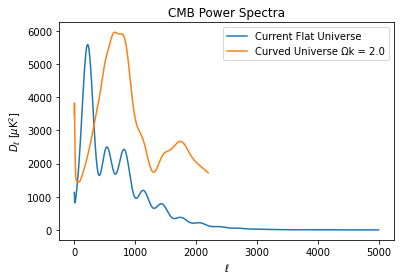
\includegraphics[width=0.8\textwidth]{images/power spectrum.png}
    \caption{A comparison of the CMB power spectrums of a flat universe and a positively curved universe.}
    \label{fig:my_label}
\end{figure}

I also generated the temperature anisotropy maps for the aforementioned curved and flat simulated universes.

\begin{figure}[H]
     \centering
     \begin{subfigure}[t]{0.49\textwidth}
         \centering
         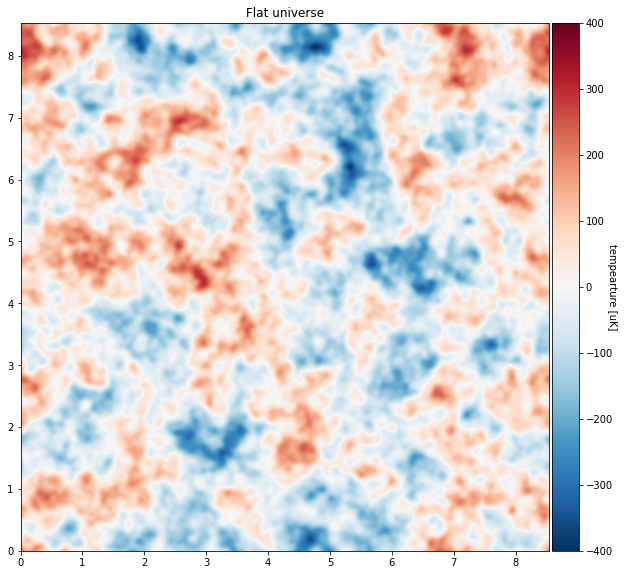
\includegraphics[width=\textwidth]{images/flat temperature anisotropy map.png}
         \caption{Flat universe}
         \label{fig:my_label}
     \end{subfigure}
     \hfill
     \begin{subfigure}[t]{0.49\textwidth}
         \centering
         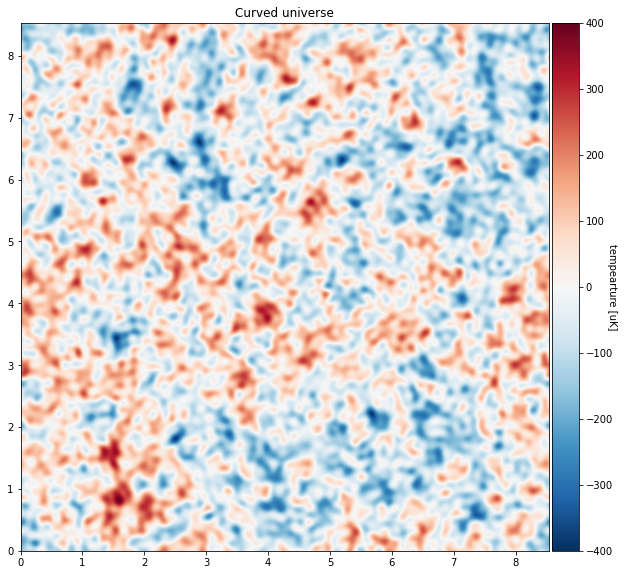
\includegraphics[width=\textwidth]{images/curved temperature anisotropy map.png}
         \caption{Curved universe $\Omega_k = 2$}
         \label{fig:my_label}
     \end{subfigure}
        \caption{Temperature Anisotropy Maps}
        \label{fig:my_label}
\end{figure}

\end{document}
